\documentclass[10pt,a4paper]{article}
% Harava admin and server guide. Built with:  pdflatex admin_guide.tex  (three times, for the contents)
% Same look as the Harava user guide and the WSPR Logger guides. Screenshots in guide_img/ (a_*.jpg).
\usepackage[T1]{fontenc}
\usepackage[utf8]{inputenc}
\usepackage{mathptmx}
\usepackage[scaled=.92]{helvet}
\usepackage{courier}
\usepackage{microtype}
\usepackage[a4paper,margin=2.0cm,top=2.3cm,bottom=2.2cm,headsep=0.5cm]{geometry}
\usepackage{graphicx}
\usepackage{xcolor}
\usepackage{booktabs}
\usepackage{tabularx}
\usepackage{array}
\usepackage{enumitem}
\usepackage{caption}
\usepackage{float}
\usepackage{fancyhdr}
\usepackage{textcomp}
\usepackage{amsmath}
\usepackage{amssymb}
\usepackage{tikz}
\usetikzlibrary{arrows.meta,positioning,fit}
\usepackage{listings}
\usepackage{xurl}
\usepackage[hidelinks]{hyperref}

\definecolor{accent}{HTML}{0369A1}
\definecolor{boxbg}{HTML}{F1F6FA}
\definecolor{warnbg}{HTML}{FFF7E8}
\definecolor{warn}{HTML}{B45309}
\definecolor{codebg}{HTML}{F4F5F7}
\definecolor{codecomment}{HTML}{6B7280}
\captionsetup{font=small,labelfont=bf,labelsep=period,justification=justified,singlelinecheck=false}
\setlist{itemsep=1.5pt,topsep=3pt,parsep=0pt}
\setlength{\parindent}{0pt}
\setlength{\parskip}{4.5pt plus 1pt}
\renewcommand{\arraystretch}{1.15}
\setcounter{tocdepth}{2}
\setlength{\emergencystretch}{3em}
\pagestyle{fancy}
\fancyhf{}
\fancyhead[L]{\small\itshape Harava --- admin and server guide}
\fancyhead[R]{\small\itshape Version 1.0 --- November 2026}
\fancyfoot[C]{\small\thepage}
\renewcommand{\headrulewidth}{0.3pt}
\hypersetup{pdftitle={Harava - Admin and server guide},pdfauthor={Otso Laakso, OH2GAX}}

\lstdefinestyle{sh}{basicstyle=\ttfamily\small,backgroundcolor=\color{codebg},frame=none,
  xleftmargin=6pt,xrightmargin=6pt,aboveskip=5pt,belowskip=6pt,columns=fullflexible,keepspaces=true,
  breaklines=true,breakatwhitespace=true,showstringspaces=false,upquote=true,
  comment=[l]{\#},commentstyle=\color{codecomment}\itshape,literate={~}{{\textasciitilde}}1}
\lstnewenvironment{cmd}{\lstset{style=sh}}{}

\newcommand{\ui}[1]{\textsf{\small #1}}
\newcommand{\lead}[1]{\textbf{#1}\enspace}
\newcommand{\fig}[3]{\begin{figure}[H]\centering\includegraphics[width=#2\textwidth]{guide_img/#1}\caption{#3}\end{figure}}
\newcommand{\infobox}[2]{\par\smallskip\noindent\fcolorbox{accent!60}{boxbg}{\begin{minipage}{\dimexpr\textwidth-2\fboxsep-2\fboxrule\relax}\small
  \textbf{#1}\enspace #2\end{minipage}}\par\smallskip}
\newcommand{\warnbox}[2]{\par\smallskip\noindent\fcolorbox{warn!60}{warnbg}{\begin{minipage}{\dimexpr\textwidth-2\fboxsep-2\fboxrule\relax}\small
  \textbf{#1}\enspace #2\end{minipage}}\par\smallskip}

\begin{document}
\thispagestyle{plain}
\begin{center}
{\small Harava project \quad$\cdot$\quad Admin and server guide, version 1.3 \quad$\cdot$\quad 9 November 2026}\par\vspace{10pt}
{\LARGE\bfseries Harava on a Server}\par\vspace{5pt}
{\large\bfseries Installing Harava next to other sites with nginx and Let's Encrypt,\\ users and permissions, updating, backups and troubleshooting}\par\vspace{8pt}
{\normalsize Otso Laakso (OH2GAX)}\par
{\small Example: \texttt{harava.oh2gax.org} on an AWS Ubuntu 24.04 LTS server that also runs WSPR Logger}
\end{center}
\vspace{2pt}

\infobox{In short.}{Harava is a Flask program. On your own computer it opens without a sign-in. On a server it runs as a \emph{systemd} service on \texttt{127.0.0.1:5057}, and \emph{nginx} --- the same nginx that already serves your other sites --- passes \texttt{https://harava.oh2gax.org} to it, with a free Let's Encrypt certificate. Every page then needs a sign-in, and every user has one permission: \emph{View only}, \emph{Analyze} or \emph{Admin}.
\begin{itemize}[leftmargin=1.2em]
\item Section~\ref{sec:how}: how the parts fit together, and what the installation adds and does \emph{not} change;
\item Section~\ref{sec:install}: the installation, step by step, with every command;
\item Section~\ref{sec:users}: users, permissions and the Maintenance page;
\item Section~\ref{sec:update}: updating with \texttt{update.sh}, the same way as WSPR Logger;
\item Section~\ref{sec:workbench}: the Workbench, where unknown radios become rules on the server;
\item Sections~\ref{sec:backup}--\ref{sec:quick}: backups, security, troubleshooting and a quick reference.
\end{itemize}}

\tableofcontents
\bigskip

% ─────────────────────────────────────────────────────────────────────
\section{How Harava runs on a server}\label{sec:how}

\begin{figure}[H]\centering
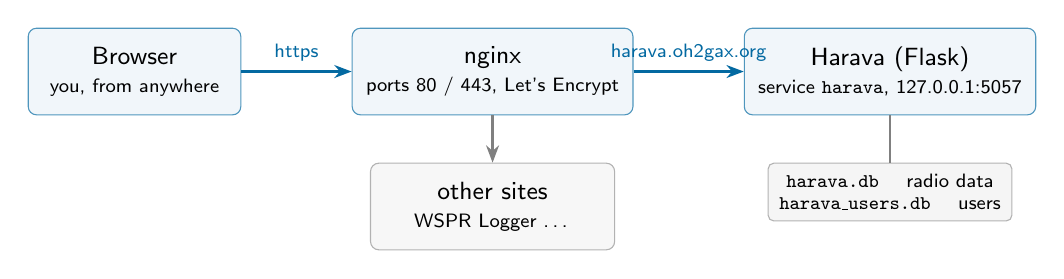
\begin{tikzpicture}[font=\sffamily\small, box/.style={draw=accent!70, fill=boxbg, rounded corners=3pt, align=center, minimum height=11mm, inner sep=5pt},
  db/.style={draw=gray!60, fill=gray!8, rounded corners=2pt, align=center, font=\sffamily\scriptsize, inner sep=4pt}, ar/.style={-{Stealth[length=2.2mm]}, thick, accent}]
\node[box, minimum width=27mm] (br) {Browser\\[-1pt]\scriptsize you, from anywhere};
\node[box, minimum width=34mm, right=14mm of br] (ng) {nginx\\[-1pt]\scriptsize ports 80 / 443, Let's Encrypt};
\node[box, minimum width=31mm, right=14mm of ng] (hv) {Harava (Flask)\\[-1pt]\scriptsize service \texttt{harava}, 127.0.0.1:5057};
\node[box, minimum width=31mm, below=6mm of ng, draw=gray!60, fill=gray!6] (other) {other sites\\[-1pt]\scriptsize WSPR Logger \dots};
\node[db, below=6mm of hv] (dbs) {\texttt{harava.db} \quad radio data\\ \texttt{harava\_users.db} \quad users};
\draw[ar] (br) -- node[above, font=\sffamily\scriptsize]{https} (ng);
\draw[ar] (ng) -- node[above, font=\sffamily\scriptsize]{harava.oh2gax.org} (hv);
\draw[ar, gray] (ng) -- (other);
\draw[thick, gray] (hv) -- (dbs);
\end{tikzpicture}
\caption{Only nginx is reachable from the internet. It sends the requests for \texttt{harava.oh2gax.org} to Harava and the others to their own programs, as before.}
\end{figure}

\lead{What the installation adds.} A folder \texttt{\textasciitilde/harava} (the program, its settings and databases), the service file \nolinkurl{/etc/systemd/system/harava.service}, one nginx site file \nolinkurl{/etc/nginx/sites-available/harava.oh2gax.org} with its link in \texttt{sites-enabled}, and a certificate for \texttt{harava.oh2gax.org}.

\lead{What it does not change.} The other nginx sites and their certificates, the other services (WSPR Logger runs on its own port, 5008), the firewall and the AWS security group: Harava listens only on \texttt{127.0.0.1}, so no new port is opened. Every nginx change is tested with \texttt{nginx -t} before nginx is \emph{reloaded} (not restarted); if the test fails, nginx keeps running with the old setup.

\begin{table}[H]\small\centering
\caption{The files of a server installation. Only the first group comes from GitHub; the rest are local and never in git.}
\begin{tabularx}{\textwidth}{>{\ttfamily\raggedright}p{5.4cm}X}
\toprule
\normalfont\textbf{File} & \textbf{What it is}\\
\midrule
harava.py, templates/, static/ & the program (from GitHub)\\
deploy/harava.service & the systemd unit to copy (from GitHub)\\
deploy/harava.oh2gax.org.nginx & the nginx site to copy (from GitHub)\\
update.sh & the update script (from GitHub)\\
\midrule
config.ini & the server's settings (Section~\ref{sec:config})\\
api\_keys.py & the CARTO map key\\
harava.db & the radio data: imports and My devices\\
harava\_users.db & users, permission, password hashes and the sign-in log\\
.harava\_secret & the random key that signs the sign-in cookies\\
data/ & Fieldwatch exports copied to the server (optional; uploads go straight into the database)\\
venv/ & the Python environment\\
\bottomrule
\end{tabularx}
\end{table}

% ─────────────────────────────────────────────────────────────────────
\section{Installing, step by step}\label{sec:install}
Log in with SSH (the AWS console) as the user \texttt{ubuntu}. Replace the domain, the user and the folder if yours differ.

\subsection{Check first (changes nothing)}
\begin{cmd}
dig +short harava.oh2gax.org          # the server's public IP (13.60.119.254)
curl -s https://checkip.amazonaws.com # the same IP
sudo ss -ltnp | grep ':5057 ' || echo "port 5057 is free"
sudo nginx -t                         # nginx must be OK before you start
ls /etc/nginx/sites-enabled/          # your existing sites
python3 --version                     # 3.9 or newer
\end{cmd}
If port 5057 is taken, use another one in \texttt{config.ini} (step~\ref{sec:config}) and in the nginx file (step~\ref{sec:nginx}).

\subsection{Packages}
\begin{cmd}
sudo apt update
sudo apt install -y git python3-venv
certbot --version || sudo apt install -y certbot python3-certbot-nginx
\end{cmd}
nginx and certbot are already there for the other sites; nothing is upgraded or reconfigured.

\subsection{The code and a Python environment}
\begin{cmd}
cd ~
git clone https://github.com/oh2gax/harava.git
cd harava
python3 -m venv venv
venv/bin/pip install -r requirements.txt
\end{cmd}

\subsection{Settings}\label{sec:config}
\begin{cmd}
cat > config.ini <<'EOF'
[app]
host = 127.0.0.1
port = 5057
database = harava.db
watch_folder = data
open_browser = false
travel_min_m = 500
require_login = true
behind_proxy = true
session_days = 30
EOF
\end{cmd}
\begin{itemize}[leftmargin=1.2em]
\item \texttt{host = 127.0.0.1} --- only nginx on the same machine reaches Harava.
\item \texttt{require\_login = true} --- Harava refuses to start until an admin exists, so it is never on the internet without a sign-in.
\item \texttt{behind\_proxy = true} --- Harava trusts nginx's \texttt{X-Forwarded-*} headers: the sign-in log shows the real addresses, and the sign-in cookie is sent over HTTPS only.
\item \texttt{session\_days} --- how long \ui{Keep me signed in} lasts.
\end{itemize}

\subsection{The map key}
\begin{cmd}
cp ~/wspr_logger/api_keys.py ~/harava/api_keys.py   # the same key as WSPR Logger
chmod 600 ~/harava/api_keys.py
\end{cmd}

\subsection{The first admin}\label{sec:firstadmin}
\begin{cmd}
venv/bin/python harava.py --add-admin
\end{cmd}
It asks for a username, first and last name and a password (at least 12 characters, twice). The password is stored only as a hash in \texttt{harava\_users.db}. All other users are added in the browser (Section~\ref{sec:users}).

\subsection{The service}
\begin{cmd}
sudo cp deploy/harava.service /etc/systemd/system/harava.service
sudo systemctl daemon-reload
sudo systemctl enable --now harava
systemctl status harava --no-pager
curl -s http://127.0.0.1:5057/healthz        # ok
curl -sI http://127.0.0.1:5057/ | head -3    # 302, Location: /login
\end{cmd}
The unit runs \texttt{venv/bin/python harava.py --no-browser} as \texttt{ubuntu} in \texttt{/home/ubuntu/harava}, restarts it if it stops, and starts it after a reboot. It also sets \texttt{TZ=Europe/Helsinki}: the server itself runs in UTC, and without it the days would change at 2 or 3 a.m.\ Finnish time; change the zone in the unit if yours is different. If your user or folder differs, edit the copy with \nolinkurl{sudo nano /etc/systemd/system/harava.service} before \texttt{daemon-reload}. The log: \texttt{journalctl -u harava -f}.

\subsection{nginx --- this site only}\label{sec:nginx}
\begin{cmd}
sudo cp deploy/harava.oh2gax.org.nginx /etc/nginx/sites-available/harava.oh2gax.org
sudo ln -s /etc/nginx/sites-available/harava.oh2gax.org /etc/nginx/sites-enabled/
sudo nginx -t && sudo systemctl reload nginx
curl -sI http://harava.oh2gax.org/ | head -3   # 302 to /login
\end{cmd}
The file handles only \texttt{server\_name harava.oh2gax.org}, accepts uploads up to 512\,MB, waits up to 5 minutes for a big import, and passes everything to \texttt{127.0.0.1:5057}.
\warnbox{If nginx -t reports an error,}{nothing has been reloaded and the other sites keep running. Remove the link (\nolinkurl{sudo rm /etc/nginx/sites-enabled/harava.oh2gax.org}), fix the file and try again.}

\subsection{HTTPS with Let's Encrypt}
\begin{cmd}
sudo certbot --nginx -d harava.oh2gax.org
sudo nginx -t
curl -s https://harava.oh2gax.org/healthz    # ok
sudo certbot renew --dry-run                 # renewal works
\end{cmd}
Certbot gets a certificate for this one name and edits only the Harava site file: it adds the HTTPS lines and, when you choose it, the redirect from \texttt{http} to \texttt{https}. The certbot timer that already renews the other sites' certificates renews this one too.

\subsection{Check the other sites, then sign in}
\begin{cmd}
systemctl status nginx --no-pager | head -5
curl -sI https://<your WSPR Logger address>/ | head -1   # still 200
\end{cmd}
Open \url{https://harava.oh2gax.org}, sign in as the admin of step~\ref{sec:firstadmin}, add the users on \ui{Maintenance} and upload Fieldwatch exports on \ui{Imports}.

% ─────────────────────────────────────────────────────────────────────
\section{Users and permissions}\label{sec:users}

\begin{table}[H]\small\centering
\caption{The permissions. Buttons that need a permission the user does not have are not shown, and the server refuses the request anyway.}
\begin{tabularx}{\textwidth}{>{\bfseries}p{2.2cm}X}
\toprule
Permission & Can\\
\midrule
View only & see the map, the Devices list, the Phone check, the Identification page and the guides; export CSV\\
Analyze & also change the data: upload and import Fieldwatch exports, \ui{Scan folder}, switch or delete imports, edit My devices, \ui{Reload database}\\
Admin & also manage users on the Maintenance page, see and combine every user's data (\ui{Whose data} $\rightarrow$ \emph{All users}), and use the Workbench\\
\bottomrule
\end{tabularx}
\end{table}

\fig{a_maintenance.jpg}{1.0}{The Maintenance page (\texttt{/maintenance}, \ui{Maintenance} in the menu for admins). Top: the users, with their names, permission and \emph{active} switch, which take effect as soon as they are changed. Middle: adding a user. Bottom: the log of sign-ins, failed sign-ins and changes, with the address they came from.}

\lead{Each user's own data.} Every import belongs to the user who imported it, recorded on one of that user's \emph{phones}. Others do not see it unless the owner shares it (with all users or with chosen users); admins see every import. Each user's \emph{My devices} are personal. Data imported while Harava had no users (on your own computer) belongs to the first admin; when the first user is added, it moves to that admin. A removed user's imports stay, shown as \emph{removed user}, and an admin can delete them.

\lead{Adding a user.} Type a username (3--64 letters, digits or \texttt{. \_ @ -}), first and last name, choose the permission and press \ui{Add user}. Harava makes a \emph{one-time password} and shows it once (Figure~\ref{fig:temp}); give it to the user. At the first sign-in the user must choose their own password before anything else.

\begin{figure}[H]\centering
\begin{minipage}[c]{0.40\textwidth}\centering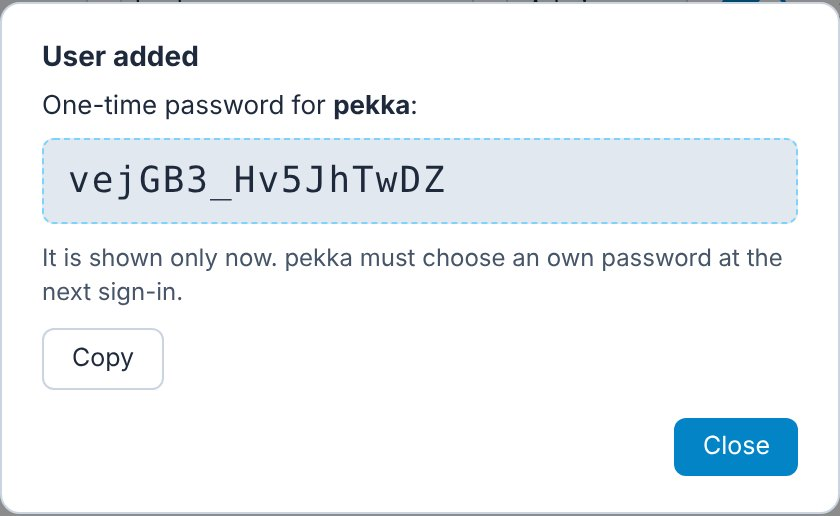
\includegraphics[width=\textwidth]{guide_img/a_temp.jpg}\end{minipage}\hfill
\begin{minipage}[c]{0.50\textwidth}\centering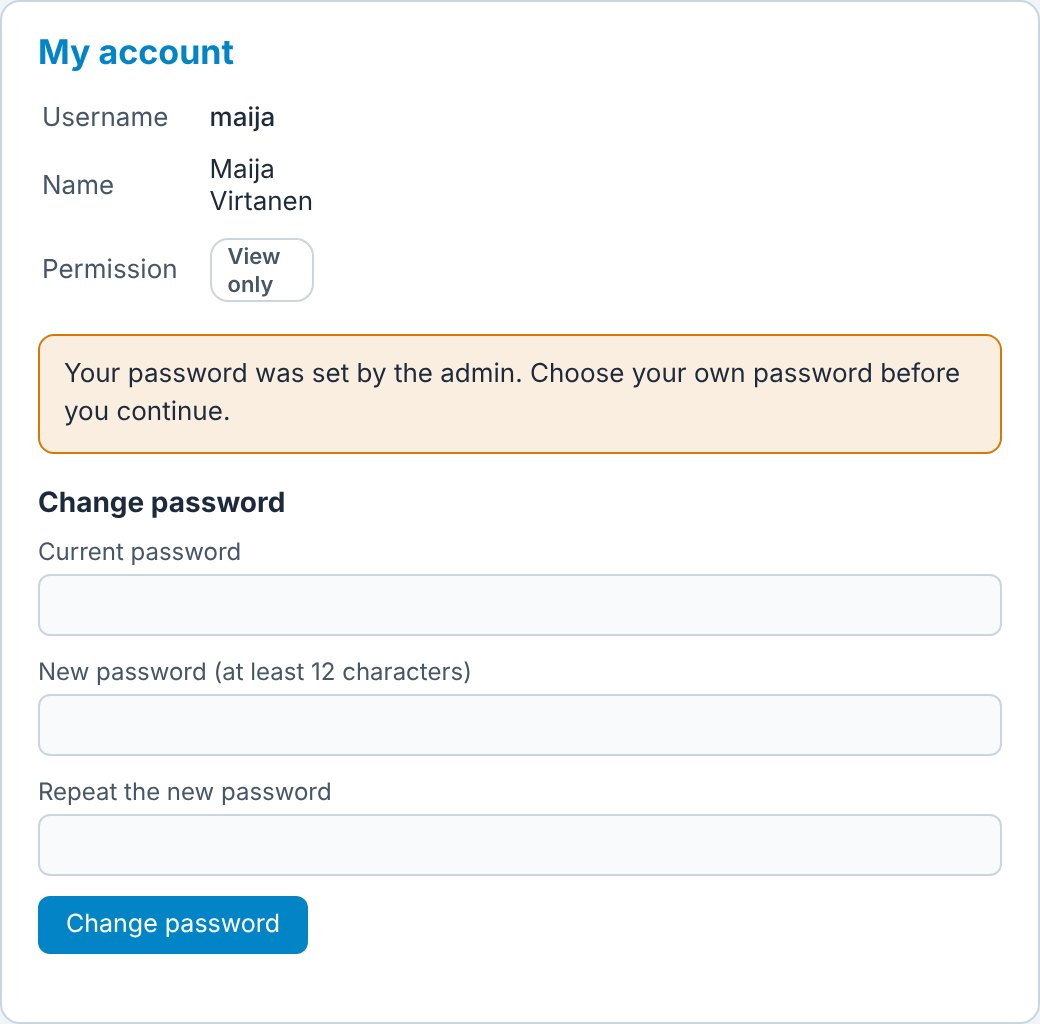
\includegraphics[width=\textwidth]{guide_img/a_account.jpg}\end{minipage}
\caption{Left: the one-time password of a new user, shown once. Right: \emph{My account} at the user's first sign-in --- the own password first.}\label{fig:temp}
\end{figure}

\lead{Changing a user.} Edit the names, the permission or the \emph{active} switch in the table. A disabled user cannot sign in, and a signed-in user is signed out at the next click. \ui{New password} makes a new one-time password (the old one stops working at once); \ui{Remove} deletes the user --- their imports and My devices stay.

\lead{Rules that keep you in.} There is always at least one active admin: the last admin cannot be removed, disabled or made View only or Analyze. Nobody can remove or disable themselves.

\lead{My account.} Every user finds \emph{My account} by clicking their name in the menu, and changes their password there. A new password signs out the user's other sessions.

\lead{Forgotten admin password.} On the server: \texttt{cd \textasciitilde/harava \&\& venv/bin/python harava.py --add-admin} with the same username sets a new password (and makes the user an admin). Then sign in again.

\lead{Failed sign-ins.} Each failed sign-in waits one second. Five from the same address within 15 minutes lock that address for the rest of the 15 minutes, and 30 from all addresses lock everyone; \texttt{sudo systemctl restart harava} clears the counters. Every failed sign-in is in the log on the Maintenance page.

% ─────────────────────────────────────────────────────────────────────
\section{Updating with update.sh}\label{sec:update}
New features come from GitHub. On the server, in the SSH console:
\begin{cmd}
bash ~/harava/update.sh
\end{cmd}
It shows the new commits and the changed files and asks \texttt{Update to <hash>? [y/N]}. After \texttt{y} it
\begin{enumerate}[leftmargin=1.5em]
\item copies \texttt{harava.db}, \texttt{harava\_users.db} and \texttt{ids/local\_rules.json} to \texttt{\textasciitilde/harava\_backups/pre\_update\_<time>/} (safe while Harava runs; the 7 newest copies are kept);
\item checks every changed Python file, page template and JSON file straight from git \emph{before} anything is changed --- if one fails, nothing changes and the old version keeps running;
\item updates the files (\texttt{git merge --ff-only}) and installs packages only if \texttt{requirements.txt} changed;
\item restarts \emph{only} the \texttt{harava} service and waits until \texttt{/healthz} answers.
\end{enumerate}

\begin{table}[H]\small\centering
\caption{The options of update.sh.}
\begin{tabularx}{\textwidth}{>{\ttfamily}p{3.6cm}X}
\toprule
\normalfont\textbf{Option} & \textbf{What it does}\\
\midrule
bash update.sh & show, ask, update, restart, check\\
bash update.sh -y & the same without asking\\
bash update.sh --rollback & go back to the version that ran before the last update, restart and check\\
SERVICE=name bash update.sh & for a service with another name\\
\bottomrule
\end{tabularx}
\end{table}

\lead{A new database format.} The version of 10 November 2026 stores every hear once per phone and links the imports to them. The first start after \texttt{update.sh} converts \texttt{harava.db} by itself, in one transaction (all or nothing; about a second for a few days of data), and the existing imports, phone and My devices become the first admin's. \texttt{bash update.sh --rollback} to an older version notices the newer format and puts back the database copy made before the update; the newer database is kept next to it as \texttt{harava.db.newer-<time>}.

\lead{Your local files are safe.} \texttt{config.ini}, \texttt{api\_keys.py}, the two databases, \texttt{.harava\_secret} and \texttt{data/} are not in git, and the script never runs \texttt{git reset}, \texttt{stash} or \texttt{checkout}. If GitHub changes a file that has also been edited on the server, it stops without changing anything and tells what to do. It also warns when \texttt{api\_keys.py} is missing, when \texttt{require\_login} is not \texttt{true}, or when there are no users. Run it as \texttt{bash update.sh}; do not \texttt{chmod +x} it (git would see the changed mode as a local edit).

% ─────────────────────────────────────────────────────────────────────
\section{The Workbench}\label{sec:workbench}
\lead{What it is.} \ui{Workbench} in the menu (\texttt{/workbench}, admins only; also a view in the phone app at \texttt{/app}) lists every Bluetooth radio of all active imports that Harava cannot name yet. Radios are put in buckets by \emph{what they advertise}, without their address and the bytes that change: the company and the first byte of the manufacturer data, service data, a vendor's own 128-bit UUID, other services and AD types --- and the shape of the name only when nothing else tells. One row is one kind of device. Three tabs: \emph{Unknown} (advertising data, no rule), \emph{Weakly identified} (company only, custom UUID only, or a low-confidence rule) and \emph{No data} (flags only).

\fig{a_workbench.jpg}{0.98}{The Workbench: progress per day at the top, the kinds on the left, one kind on the right with its status and note, the advertisement decoded, the variants and the bytes that change, hints and search links.}

\lead{Notes.} Every kind can have a status --- New, Investigating, Identified, Ignore, Can't identify --- and a note. They are stored in the table \texttt{wb\_notes} in \texttt{harava.db} and are shared by all admins; the fingerprint stays the same when rules change, so a note stays with its kind.

\lead{Rules.} \ui{Make a rule} is filled with a match that all the radios of the kind share. \ui{Preview} counts what it would catch on all days, and which already identified radios it would take over; \ui{Save rule} checks it (hex fields, UUID lists, a regular expression that compiles, a known layer, at least one condition), gives it an id starting with \texttt{local-}, and starts using it at once --- no restart.

\fig{a_wb_rule.jpg}{0.98}{Making a rule: name, layer, confidence and the suggested match, with the preview of what it would catch.}

\infobox{Where local rules live.}{In \texttt{\textasciitilde/harava/ids/local\_rules.json}, on this server only. The file is in \texttt{.gitignore}, so \texttt{update.sh} never touches it, and it copies it with the databases before every update. Local rules are tried \emph{before} the shared \texttt{ids/harava\_ids.json}. The \ui{Local rules} table at the bottom of the Workbench lists them and removes them; \ui{Export rules and notes} downloads the rules and the notes as one JSON file, so good rules can be added to the shared database in a later version of Harava.}

% ─────────────────────────────────────────────────────────────────────
\section{Backups, moving and removing}\label{sec:backup}
\lead{What to keep.} \texttt{harava.db} (also the Workbench notes), \texttt{harava\_users.db}, \texttt{ids/local\_rules.json} (the Workbench's rules), \texttt{config.ini}, \texttt{api\_keys.py} and \texttt{.harava\_secret}. \texttt{archive/} holds a compressed copy of every uploaded export (for \ui{Re-read}; \texttt{keep\_originals = false} in \texttt{config.ini} turns it off); it can be rebuilt from your own exports, so it is not part of the update backups. \texttt{update.sh} copies the databases and the local rules before every update; copy them off the server now and then, for example from your own computer:
\begin{cmd}
scp ubuntu@harava.oh2gax.org:harava_backups/pre_update_*/harava*.db .
\end{cmd}
A consistent copy while Harava runs: \texttt{sqlite3 harava.db ".backup harava\_copy.db"} (or the copies \texttt{update.sh} makes).

\lead{A snapshot for analysis.} To look at the data elsewhere --- on your computer, or together with an assistant --- use \ui{Database snapshot} on the Maintenance page instead of copying files by hand (Figure~\ref{fig:snapshot}). \ui{Make snapshot} makes a complete, consistent copy while Harava runs and downloads it as one zip: the database (\texttt{harava\_snapshot\_<date>\_<time>.db}), the Workbench's \texttt{local\_rules.json} and \texttt{snapshot\_info.json} (version, time, how many imports and hears, the time span, the owners). \emph{My data only} leaves out every other user's imports, phones and My devices completely (the copy is compacted, so nothing of them stays in the file); \emph{Everyone's data} keeps all. Save it outside the scan folder, e.g.\ in \texttt{tmp\_files}, and keep it private. The server keeps the 10 newest snapshots in \texttt{snapshots/} (readable only by the Harava user, not in git); making, downloading and deleting one is logged.

\begin{figure}[H]\centering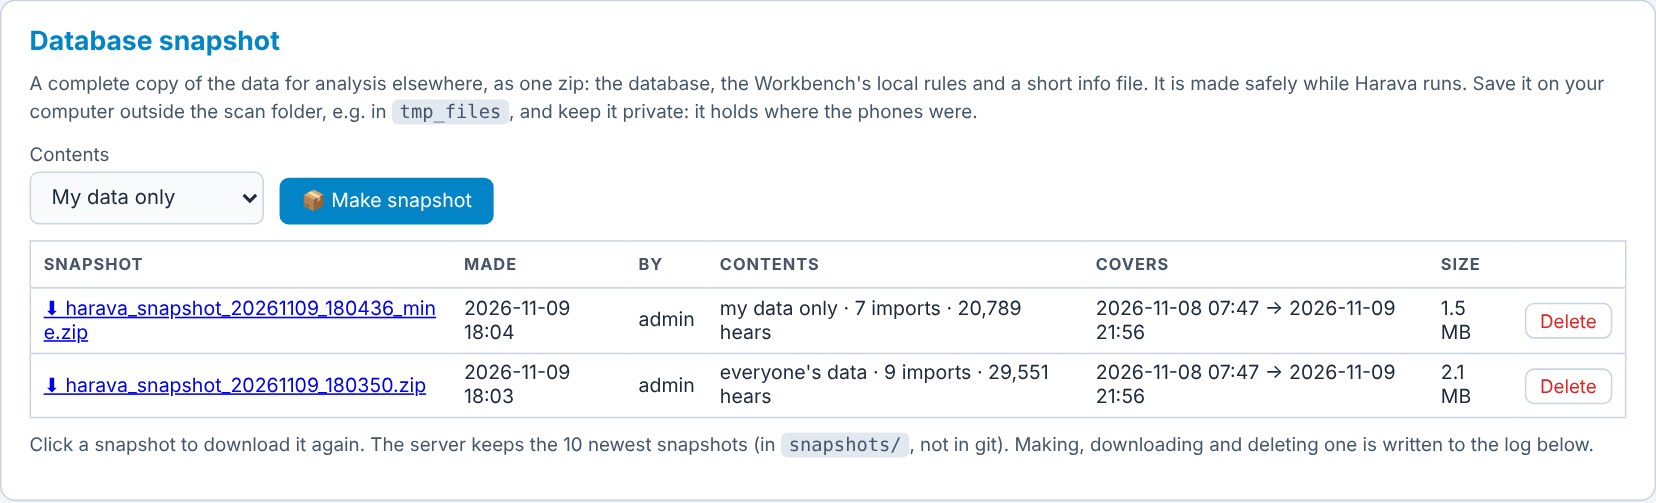
\includegraphics[width=0.98\textwidth]{guide_img/a_snapshot.jpg}
\caption{Database snapshot on the Maintenance page: one of the admin's own data and one of everyone's.}\label{fig:snapshot}\end{figure}

\lead{Moving to another server.} Install as in Section~\ref{sec:install}, but before step~\ref{sec:firstadmin} copy the six files above (and \texttt{archive/}, if you want Re-read) into \texttt{\textasciitilde/harava}; the users and the data come with them.

\lead{Removing Harava completely.}
\begin{cmd}
sudo systemctl disable --now harava
sudo rm /etc/systemd/system/harava.service
sudo rm /etc/nginx/sites-enabled/harava.oh2gax.org /etc/nginx/sites-available/harava.oh2gax.org
sudo nginx -t && sudo systemctl reload nginx
sudo certbot delete --cert-name harava.oh2gax.org
rm -rf ~/harava ~/harava_backups
\end{cmd}

% ─────────────────────────────────────────────────────────────────────
\section{Security in short}\label{sec:security}
\begin{itemize}[leftmargin=1.2em]
\item Passwords are stored only as salted hashes (Werkzeug, scrypt); a one-time password must be changed at the first sign-in; at least 12 characters.
\item The sign-in is a signed cookie (\texttt{HttpOnly}, \texttt{SameSite=Lax}, HTTPS only behind nginx); the key is random and stays on the server in \texttt{.harava\_secret}. Without \ui{Keep me signed in} it ends when the browser closes.
\item A new password, a disabled user, a removed user or a changed permission takes effect at once, also for a user who is signed in.
\item Requests that change data must come from Harava's own page; pages are sent with \texttt{no-store}, \texttt{X-Frame-Options: DENY} and \texttt{nosniff}; search engines are told not to index the site.
\item Failed sign-ins are slowed down and locked out (Section~\ref{sec:users}) and logged with their address.
\item The service runs as \texttt{ubuntu}, not as root, with \texttt{NoNewPrivileges}, a private \texttt{/tmp} and \texttt{UMask=0077}; \texttt{harava\_users.db}, \texttt{.harava\_secret} and \texttt{api\_keys.py} are readable only by that user.
\item Snapshots (Maintenance) are for admins only, are kept with file mode 0600 and are logged when made, downloaded or deleted; \emph{My data only} leaves other users' data out of the file entirely.
\item Harava stores the addresses and names of other people's radios. Keep the users few, use \ui{Mask addresses} for screenshots you share, and follow the data-protection law of your country.
\end{itemize}

% ─────────────────────────────────────────────────────────────────────
\section{Troubleshooting}\label{sec:trouble}
\begin{table}[H]\small\centering
\caption{Common problems.}
\begin{tabularx}{\textwidth}{>{\raggedright}p{4.4cm}X}
\toprule
\textbf{Symptom} & \textbf{Cause and fix}\\
\midrule
\emph{502 Bad Gateway} & Harava is not running: \texttt{systemctl status harava}, \texttt{journalctl -u harava -n 50}.\\
The service stops at once; the log says \emph{require\_login = true but there are no users yet} & Add the first admin (step~\ref{sec:firstadmin}), then \texttt{sudo systemctl restart harava}.\\
\emph{413 Request Entity Too Large} when uploading & The file is over 512\,MB: raise \texttt{client\_max\_body\_size} in the site file (and \texttt{MAX\_CONTENT\_LENGTH} in \texttt{harava.py}).\\
\emph{Too many failed sign-ins} & Wait 15 minutes, or \texttt{sudo systemctl restart harava}.\\
Forgotten admin password & \texttt{venv/bin/python harava.py --add-admin} with the same username.\\
The sign-in log shows \texttt{127.0.0.1} for everyone & \texttt{behind\_proxy = true} is missing from \texttt{config.ini}.\\
Signed out after every click & The site is opened over \texttt{http} while \texttt{behind\_proxy = true}: open \texttt{https://}, or let certbot add the redirect.\\
The map has an ``API key required'' watermark & \texttt{api\_keys.py} is missing or has no key.\\
\texttt{nginx -t} warns \emph{protocol options redefined for 0.0.0.0:443} (or \texttt{[::]:443}) after certbot & Another site writes its \texttt{listen 443} line differently, e.g.\ with \texttt{http2}. Make Harava's lines match the other sites' (for example \texttt{listen [::]:443 ssl http2;} and \texttt{listen 443 ssl;}), then \texttt{sudo nginx -t \&\& sudo systemctl reload nginx}. The warning itself is harmless.\\
Days or times are 2--3 hours off & The server runs in UTC: the unit needs \texttt{Environment=TZ=Europe/Helsinki}. Copy the unit again, \texttt{sudo systemctl daemon-reload}, \texttt{sudo systemctl restart harava}.\\
\texttt{update.sh}: \emph{GitHub changes file(s) that are also modified on this machine} & A file from git was edited on the server: copy it aside, \texttt{git checkout -- <file>}, run \texttt{update.sh} again.\\
\bottomrule
\end{tabularx}
\end{table}

% ─────────────────────────────────────────────────────────────────────
\section{Quick reference}\label{sec:quick}
\begin{table}[H]\small\centering
\begin{tabularx}{\textwidth}{>{\raggedright}p{4.4cm}>{\ttfamily\small}X}
\toprule
\textbf{I want to \dots} & \normalfont\textbf{Command}\\
\midrule
update Harava & bash \textasciitilde/harava/update.sh\\
go back after an update & bash \textasciitilde/harava/update.sh --rollback\\
see if it runs & systemctl status harava\\
read its log & journalctl -u harava -f\\
restart it & sudo systemctl restart harava\\
add an admin / reset a password & cd \textasciitilde/harava \&\& venv/bin/python harava.py --add-admin\\
test nginx and reload it & sudo nginx -t \&\& sudo systemctl reload nginx\\
test the renewal & sudo certbot renew --dry-run\\
check that Harava answers & curl -s https://harava.oh2gax.org/healthz\\
\bottomrule
\end{tabularx}
\caption{Commands on the server.}
\end{table}

\vfill
{\small Harava is MIT licensed: \url{https://github.com/oh2gax/harava}. This guide was written with the assistance of Claude (Anthropic).}

\end{document}
